\section{Proposed Methodology}
\label{sec:method}

\begin{figure*}[t]
\centering
\begin{tikzpicture}[
    node distance=0.45cm and 0.55cm,
    box/.style={rectangle, rounded corners=3pt, draw=black!75, thick, align=center, font=\scriptsize, minimum height=0.82cm, inner sep=3.5pt},
    ipbox/.style={box, fill=blue!8},
    lstmBox/.style={box, fill=orange!10},
    posebox/.style={box, fill=teal!9},
    fusebox/.style={box, fill=purple!10, font=\scriptsize\bfseries},
    arrow/.style={-{Stealth[scale=0.85]}, thick, draw=black!75}
]
    % Input
    \node[box, fill=gray!15, minimum width=2.1cm, minimum height=2.9cm, font=\scriptsize\bfseries] (vid) {Input Broadcast\\Cricket Video\\$\{I_t\}_{t=1}^{N}$\\[3pt](.avi / .mp4)};

    % Approach 1: Classical IP
    \node[ipbox, right=0.65cm of vid, yshift=1.15cm, minimum width=2.65cm] (ip1) {\textbf{Approach 1: Classical IP}\\1. CIE-LAB CLAHE ($\gamma=2.5$)\\2. HSV Turf/Pitch Crowd Mask};
    \node[ipbox, right=0.45cm of ip1, minimum width=2.95cm] (ip2) {3. Bobick--Davis MHI $H_\tau$\\4. Pan-Comp.\ Farneb\"{a}ck Flow\\(36-Bin Polar HOOF)};
    \node[ipbox, right=0.45cm of ip2, minimum width=2.75cm] (ip3) {5. Canny Edges + Hough\\Bat Angle Hist.\ (18-Bin)\\+ MHI-HOG (102-D Vec)};
    \node[fusebox, right=0.45cm of ip3, minimum width=2.65cm] (ip4) {CricIP-FusionNet\\(GCAM 3-Stream Gate)\\$\sim$1.28\,s CPU Inference};

    % Approach 2: ResNet50 + LSTM
    \node[lstmBox, right=0.65cm of vid, yshift=0.0cm, minimum width=2.65cm] (l1) {\textbf{Approach 2: CNN-LSTM}\\Uniform 16-Frame Sampling\\($224\times224$ Norm.\ RGB)};
    \node[lstmBox, right=0.45cm of l1, minimum width=2.95cm] (l2) {Pretrained ResNet50\\(Layers 1--3 Frozen,\\Layer-4 Fine-Tuned)};
    \node[lstmBox, right=0.45cm of l2, minimum width=2.75cm] (l3) {Sequential 128-D LSTM\\(\texttt{dropout=0.4})\\Temporal State $h_T$};
    \node[fusebox, right=0.45cm of l3, minimum width=2.65cm] (l4) {10-Class Softmax\\(79.0\% CricShot10\\Test Accuracy)};

    % Approach 3: Pose-Guided Dual-GRU
    \node[posebox, right=0.65cm of vid, yshift=-1.15cm, minimum width=2.65cm] (p1) {\textbf{Approach 3: Pose-Guided}\\YOLO11m-Pose + Bat Det.\\+ Viterbi Striker Tracker};
    \node[posebox, right=0.45cm of p1, minimum width=2.95cm] (p2) {2-Pass Striker Crop + Seg.\\+ 68-D Torso-Normalized\\Biomechanical Pose Vec};
    \node[posebox, right=0.45cm of p2, minimum width=2.75cm] (p3) {Wrist-Speed Impact Warp\\($K=15$ Frames, Impact $k^*=8$)\\+ Mirrored EfficientNetV2-S};
    \node[fusebox, right=0.45cm of p3, minimum width=2.65cm] (p4) {Dual-GRU Fusion\\(78.72\% Acc / 77.90\%\\Macro-F1 on CricShot10k)};

    % Arrows
    \draw[arrow] (vid.east) -- ++(0.25,0) |- (ip1.west);
    \draw[arrow] (vid.east) -- (l1.west);
    \draw[arrow] (vid.east) -- ++(0.25,0) |- (p1.west);

    \draw[arrow] (ip1) -- (ip2);
    \draw[arrow] (ip2) -- (ip3);
    \draw[arrow] (ip3) -- (ip4);

    \draw[arrow] (l1) -- (l2);
    \draw[arrow] (l2) -- (l3);
    \draw[arrow] (l3) -- (l4);

    \draw[arrow] (p1) -- (p2);
    \draw[arrow] (p2) -- (p3);
    \draw[arrow] (p3) -- (p4);
\end{tikzpicture}
\caption{\textbf{Overview of the three progressive approaches explored in this work.} \textbf{Top (Approach 1):} A 6-stage Classical Image Processing pipeline extracting explicit illumination-normalized keyframes, crowd-suppressed ROIs, Bobick--Davis MHI, pan-compensated HOOF, and Canny--Hough bat geometry fused via Gated Cross-Modal Attention. \textbf{Middle (Approach 2):} An end-to-end spatio-temporal ResNet50 + LSTM network over 16 RGB frames. \textbf{Bottom (Approach 3):} Our large-scale Pose-Guided Striker Isolation and Impact-Aligned Dual-GRU fusion architecture evaluated on 10,091 clips.}
\label{fig:overview}
\end{figure*}

\Cref{fig:overview} shows the overall workflow of our project. We designed and tested three progressive pipelines to understand the strengths and limitations of classical image processing, end-to-end CNN-LSTM sequence learning, and pose-guided biomechanical fusion. Below we explain each step and why it was chosen.

% =============================================================================
\subsection{Approach 1: Classical Image Processing and Motion-Geometry Pipeline}
\label{sec:method_ip}

Our first approach focuses on extracting explicit, physically interpretable image processing features from broadcast videos so that the model relies on bat geometry and swing motion rather than stadium background colors. Given a video clip, we sample $T=8$ uniformly spaced keyframes from the central 80\% active window and pass them through five classical image processing stages (\Cref{fig:ip_stages}):

\paragraph{Stage 1: CIE-LAB Luminance CLAHE (Why: Illumination Normalization).}
Broadcast cricket clips suffer from strong contrast variations between sunlit turf and helmet/body shadows. Applying histogram equalization directly to R, G, and B channels distorts the color of the grass and pitch. Instead, we convert each frame to the perceptually uniform CIE-LAB color space and apply Contrast Limited Adaptive Histogram Equalization (CLAHE)~\cite{zuiderveld1994contrast} only to the luminance channel $L^*$ ($8\times8$ tiles, clip limit $\gamma=2.5$), then convert back to RGB. This brightens the batter and bat edges under shadows without changing the chromaticity $(a^*, b^*)$.

\paragraph{Stage 2: HSV Turf/Pitch Segmentation and Crowd Suppression (Why: Removing Spectator \& Scoreboard Clutter).}
To stop moving spectators in the upper stands and TV scoreboards at the bottom from distracting the classifier, we convert the CLAHE frame to HSV space and segment the green outfield ($H\in[28,95], S\in[30,255], V\in[35,255]$) and the tan clay pitch strip ($H\in[10,28], S\in[20,170], V\in[80,255]$). We apply morphological closing ($15\times15$ ellipse) to fill holes inside the batter's silhouette and morphological opening ($5\times5$ ellipse) to remove noise:
\begin{equation}
    M_{\text{field}} = \big((M_{\text{green}} \cup M_{\text{pitch}}) \bullet B_{15}\big) \circ B_{5}.
\end{equation}
We blend $M_{\text{field}}$ with a centered 2D Gaussian batter prior $G(x,y)$ so the batter's head and raised bat are preserved while background crowd regions are darkened by 80\%. We also record a 6-D vector of HSV field/pitch statistics.

\paragraph{Stage 3: Bobick--Davis Motion History Image (Why: Capturing the Swing Arc in One 2D Map).}
To summarize the entire temporal swing trajectory into a single 2D image, we compute the recursive Motion History Image (MHI) $H_\tau(x,y,t)$~\cite{bobick2001recognition} from morphologically cleaned frame-difference silhouettes $\Psi(x,y,t)$ (threshold $\xi=22$, masking out the top 18\% crowd banner and bottom 18\% scoreboard ticker):
\begin{equation}
    H_\tau(x,y,t) = \begin{cases}
    \tau & \text{if } \Psi(x,y,t) = 1, \\
    \max\big(0, H_\tau(x,y,t-1) - 1\big) & \text{otherwise},
    \end{cases}
\end{equation}
with decay $\tau=8$. Bright pixels in $H_\tau$ represent the most recent position of the bat and arms, while darker trails show the earlier backlift and downswing path.

\begin{figure*}[t]
\centering
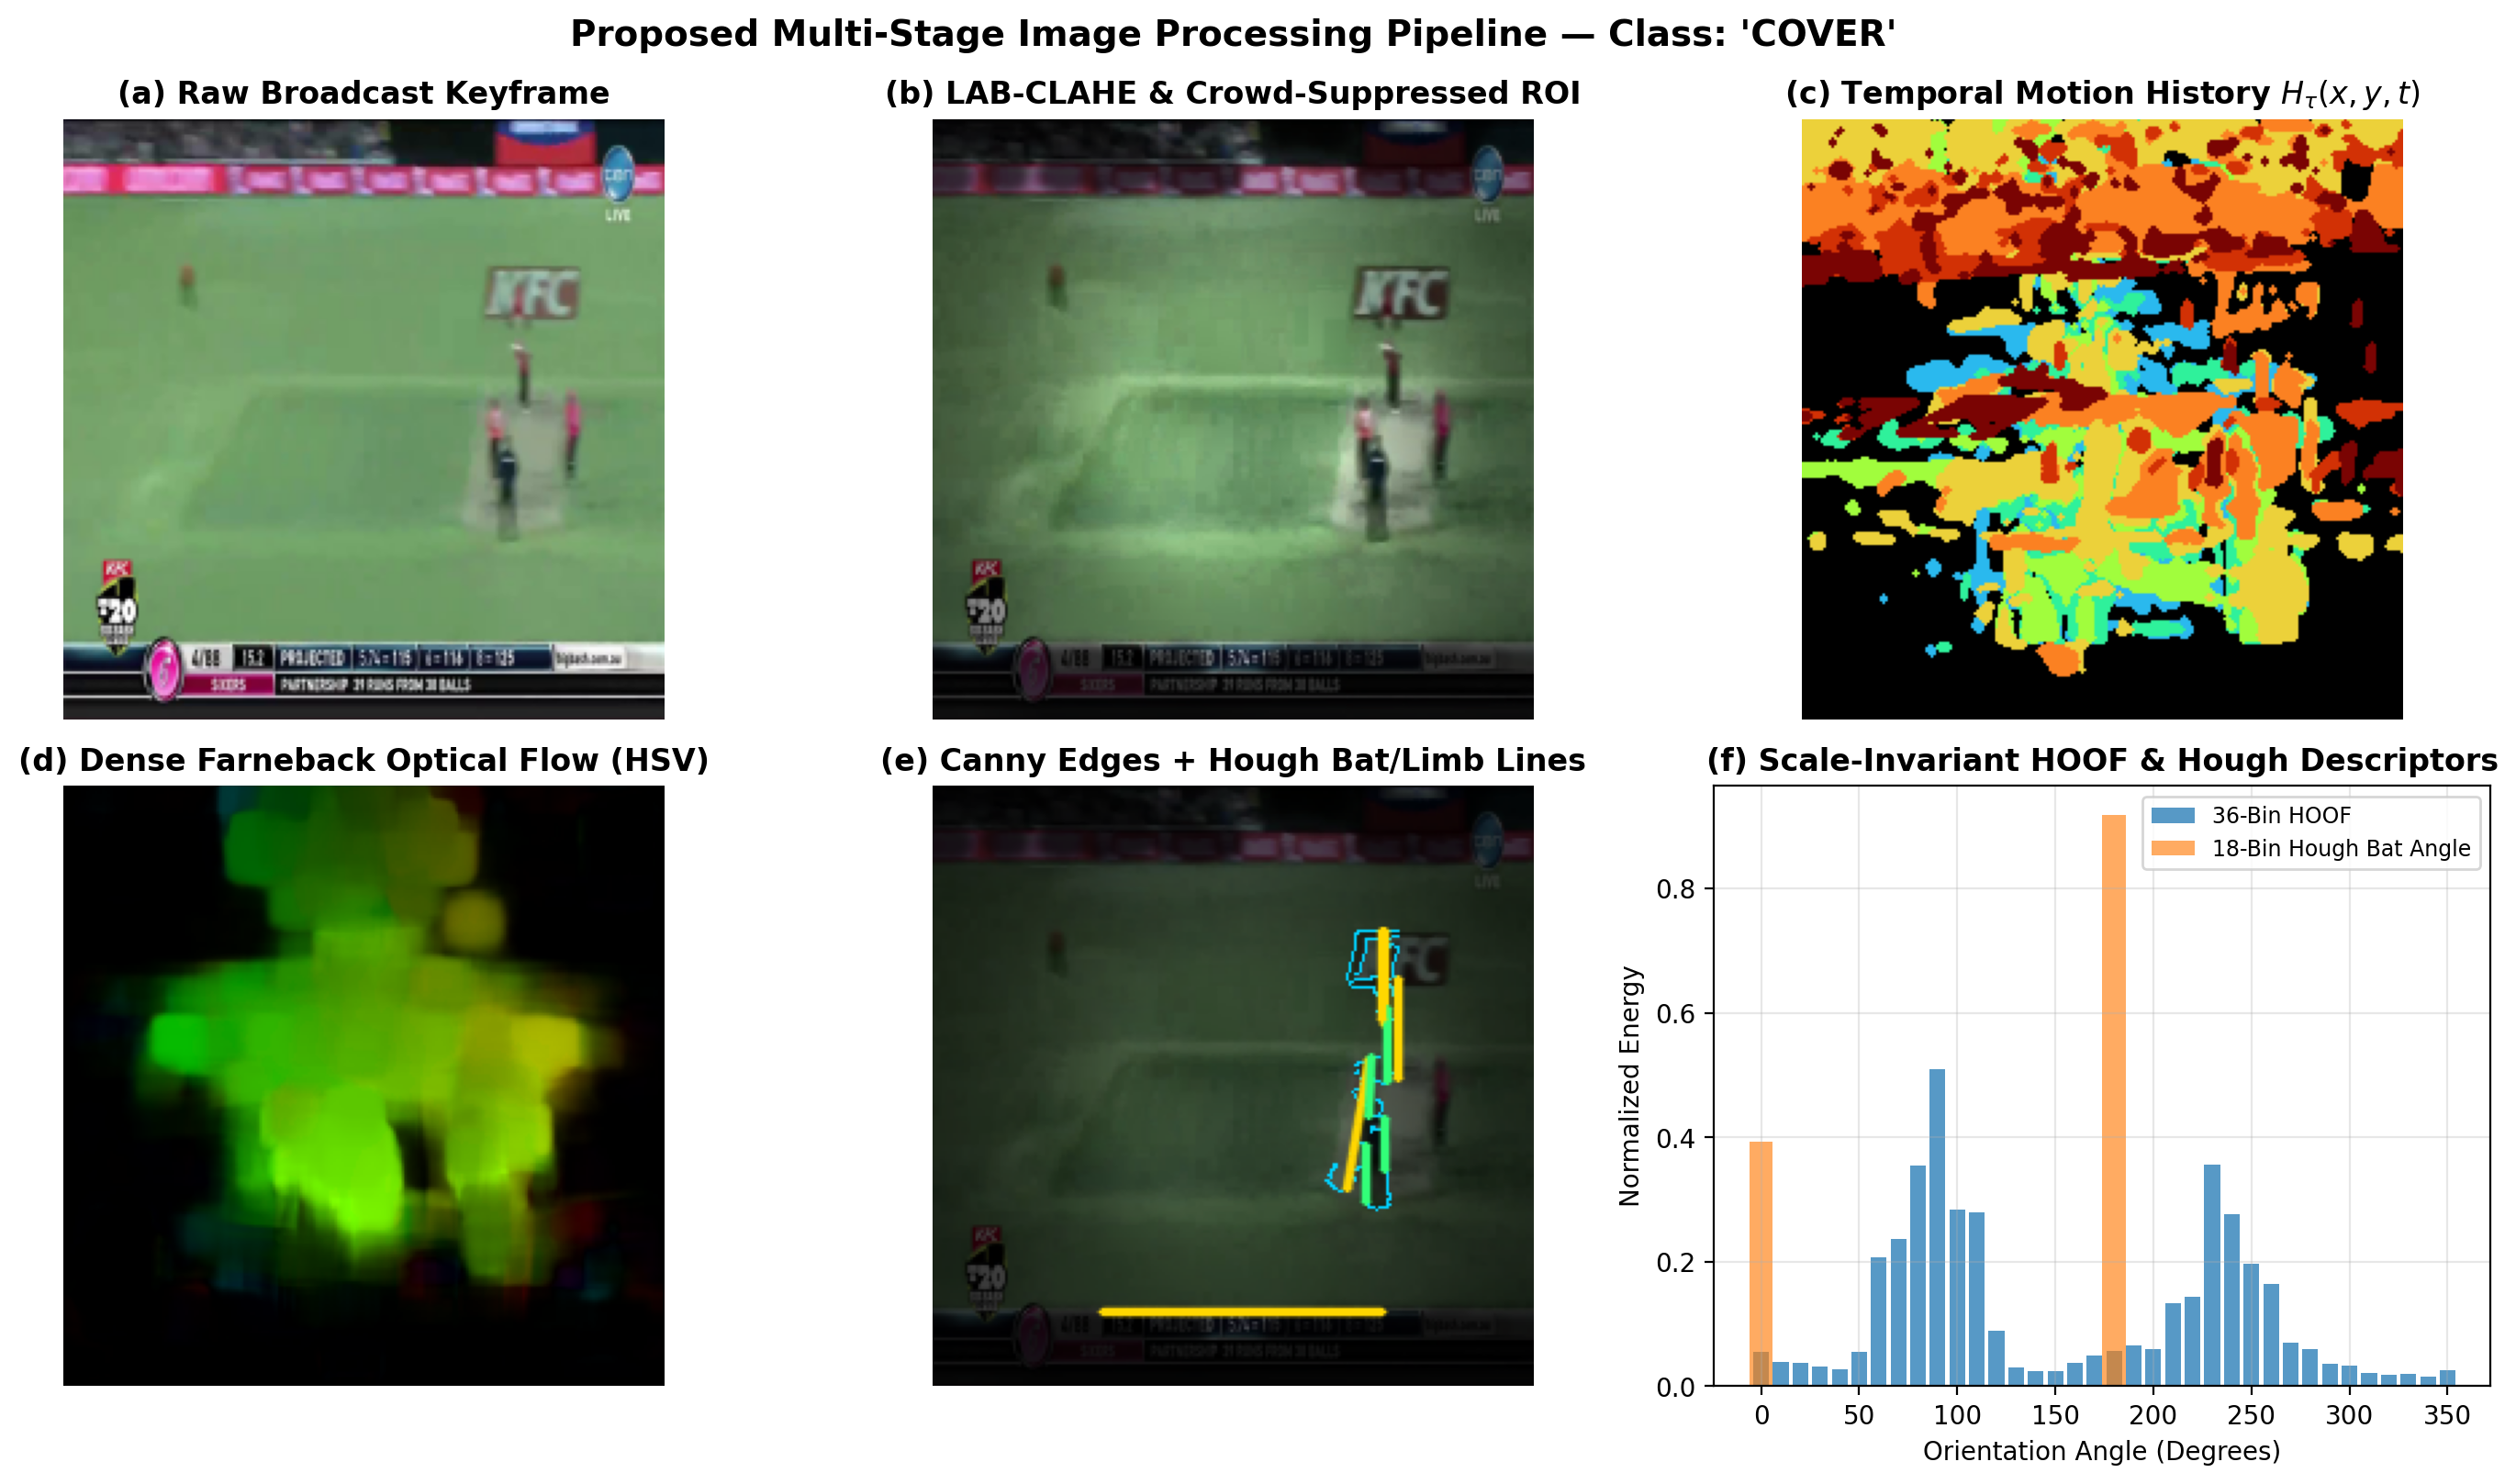
\includegraphics[width=0.98\textwidth]{fig_ip_pipeline.png}
\caption{\textbf{Output of our 6-stage Classical Image Processing pipeline on a real broadcast \textit{Cover Drive} clip from CricShot10.} \textbf{(a)} Raw frame; \textbf{(b)} Stage 1 CIE-LAB CLAHE; \textbf{(c)} Stage 2 HSV turf/pitch mask and crowd suppression; \textbf{(d)} Stage 3 Bobick--Davis MHI $H_\tau(x,y,t)$; \textbf{(e)} Stage 4 camera-pan-compensated Farneb\"{a}ck optical flow (HSV wheel); \textbf{(f)} Stage 5 adaptive Canny edges (cyan) and Probabilistic Hough bat/limb lines (gold/green).}
\label{fig:ip_stages}
\end{figure*}

\paragraph{Stage 4: Camera-Pan-Compensated Optical Flow and 36-Bin Polar HOOF (Why: Separating Bat Motion from Camera Pan).}
When the camera pans to follow the ball, every pixel in the frame moves. To isolate the batter's motion from the camera's pan, we compute dense Farneb\"{a}ck optical flow~\cite{farneback2003two} $(u,v)$ between consecutive frames and subtract the median flow vector $(\bar{u}_{\text{bg}}, \bar{v}_{\text{bg}})$ estimated from a 16-pixel border ring around the frame edges:
\begin{equation}
    \tilde{u}(x,y) = u(x,y) - \bar{u}_{\text{bg}}, \qquad \tilde{v}(x,y) = v(x,y) - \bar{v}_{\text{bg}}.
\end{equation}
Converting $(\tilde{u}, \tilde{v})$ to polar magnitude $M(x,y)$ and direction $\theta(x,y) \in [0, 2\pi)$, we accumulate a magnitude-weighted 36-bin Histogram of Oriented Optical Flow (HOOF) ($10^\circ$ per bin) normalized to unit $L_2$ norm, plus 4 global kinematic ratios ($\mathbb{E}[M]$, $\text{Std}[M]$, horizontal-to-vertical energy ratio, and active motion fraction), giving a 40-D motion vector.

\paragraph{Stage 5: Canny--Hough Bat Angle Histogram and MHI-HOG (Why: Explicit Bat Orientation).}
Different strokes have very distinct bat angles at impact (e.g., vertical $80^\circ$--$100^\circ$ for \textit{Defense} and \textit{Straight Drive}, vs.\ horizontal $15^\circ$--$45^\circ$ for \textit{Pull}, \textit{Hook}, and \textit{Cut}). We run adaptive Canny edge detection (thresholds $0.66\,\text{med}(I)$ and $1.33\,\text{med}(I)$) inside the batter ROI and apply the Probabilistic Hough Transform ($\rho=1$\,px, $\theta=1^\circ$, min length 16\,px). To prevent the horizontal white popping crease on the pitch from being mistaken for a horizontal bat, we filter out strictly horizontal segments ($<8^\circ$ or $>172^\circ$) and bin the remaining line lengths into an 18-bin orientation histogram over $[0^\circ, 180^\circ)$, supplemented by angular entropy, dominant angle, and a 36-D spatial HOG descriptor on the $64\times64$ MHI+Edge map. Concatenating all features yields an explicit \textbf{102-D classical IP vector} $\mathbf{f}_{\text{IP}} \in \mathbb{R}^{102}$.

\paragraph{Stage 6: Gated Cross-Modal Attention Fusion (\textbf{CricIP-FusionNet}).}
Finally, we fuse three streams—Stream~1 (CLAHE + crowd-suppressed keyframes encoded via a ResNet-18 + temporal attention pool $\rightarrow \mathbf{e}_{\text{rgb}} \in \mathbb{R}^{256}$), Stream~2 (3-channel composite motion map $[\text{MHI}, \text{Flow}, \text{MEI}]$ encoded via ResNet-18 $\rightarrow \mathbf{e}_{\text{mot}} \in \mathbb{R}^{256}$), and Stream~3 ($\mathbf{f}_{\text{IP}} \in \mathbb{R}^{102}$ projected via a 2-layer MLP $\rightarrow \mathbf{e}_{\text{geom}} \in \mathbb{R}^{256}$)—using a Gated Cross-Modal Attention Module (GCAM) that predicts sample-specific gating weights $[\alpha_{\text{rgb}}, \alpha_{\text{mot}}, \alpha_{\text{geom}}] = \text{Softmax}(W_g[\mathbf{e}_{\text{rgb}} \| \mathbf{e}_{\text{mot}} \| \mathbf{e}_{\text{geom}}])$.

% =============================================================================
\subsection{Approach 2: End-to-End Spatio-Temporal ResNet50 + LSTM}
\label{sec:method_lstm}

While Classical IP excels on strokes with clear bat geometry (\textit{Defense}, \textit{Straight Drive}, \textit{Lofted}, \textit{Sweep}), fast wrist strokes (\textit{Flick}, \textit{Late Cut}, \textit{Hook}) often suffer from motion blur on the bat blade. To test how an end-to-end deep sequence model performs without handcrafted edges, we implemented a spatio-temporal \textbf{ResNet50 + LSTM} architecture:
\begin{enumerate}
    \item \textbf{Uniform Temporal Sampling ($T=16$ Frames):} We sample 16 uniformly spaced RGB frames across each video clip, resize them to $224\times224$, and normalize with ImageNet mean and standard deviation.
    \item \textbf{Selective Layer-4 ResNet50 Fine-Tuning (Why: Preventing Overfitting):} Using an ImageNet-pretrained ResNet50, we freeze the early convolutional blocks (\texttt{conv1} through \texttt{layer3}) so general edge and texture filters are preserved, and fine-tune only \texttt{layer4} to adapt high-level spatial representations ($\mathbf{v}_t \in \mathbb{R}^{2048}$) to cricket postures.
    \item \textbf{LSTM Temporal Modeling and Regularization:} The sequence $\{\mathbf{v}_t\}_{t=1}^{16}$ is passed through a 128-unit LSTM layer followed by dropout regularization (\texttt{dropout=0.4}) and a fully connected 10-class linear classification head ($\mathbb{R}^{128} \rightarrow \mathbb{R}^{10}$) operating on the final temporal state $\mathbf{h}_{16}$.
\end{enumerate}

% =============================================================================
\subsection{Approach 3: Pose-Guided Striker Isolation and Biomechanical Dual-GRU Fusion}
\label{sec:method_pose}

When scaling up to the 15-class, 10,091-clip \textbf{CricShot10k} benchmark, we found that full-frame models (like Approach~2) lose accuracy because other people on the field (bowler, umpire, non-striker) enter the frame and because the impact moment varies widely across clips. Approach~3 solves both issues through a three-stage pose-guided pipeline:

\begin{figure*}[t]
\centering
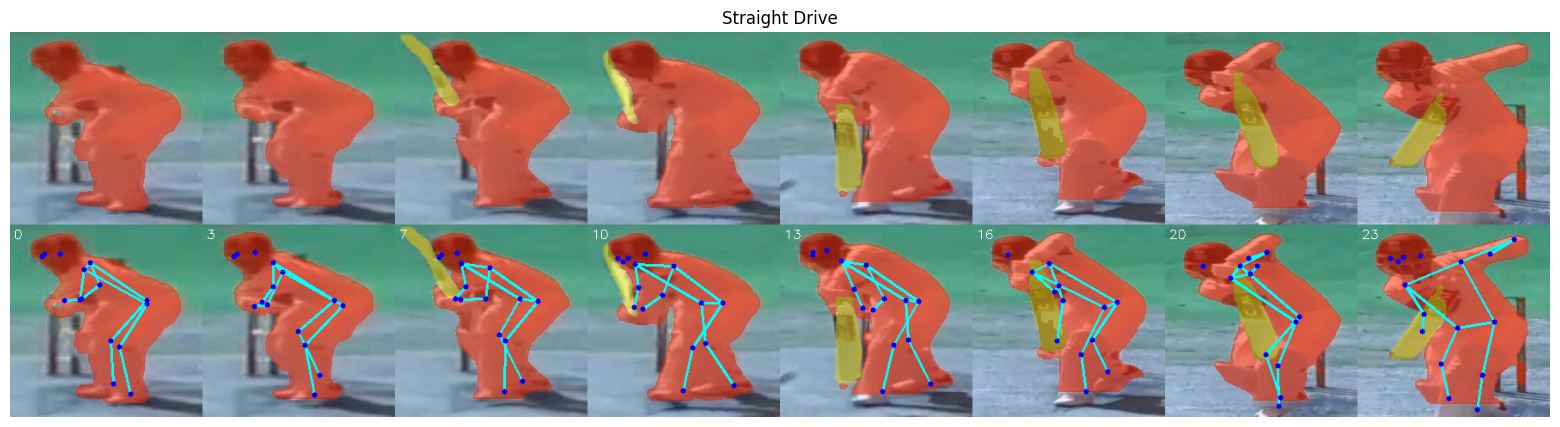
\includegraphics[width=0.98\textwidth]{fig_striker_seg_pose.png}
\caption{\textbf{Stage 1 of Approach 3 (Viterbi Striker Isolation and 2-Pass YOLO11m-Pose Refinement).} \textbf{Top row:} Striker + bat union crop ($224\times224$) with segmentation overlay removing the bowler, umpire, and non-striker. \textbf{Bottom row:} Refined 17-keypoint COCO skeleton tracked across the stroke.}
\label{fig:striker_pose}
\end{figure*}

\paragraph{1. Viterbi Dynamic Programming Striker Tracker and 2-Pass Pose Refinement (Why: Isolating Only the Batter).}
In each frame $t$, we run \texttt{YOLO11m-pose} (detecting all people and their 17 COCO keypoints) and a YOLO bat detector. Because 4--6 people may be detected per frame, we score each candidate person $i$ using a unary striker score $S_t(i)$ combining box area, horizontal closeness to the pitch center, keypoint confidence, and wrist-to-bat proximity. We then solve for the globally optimal striker trajectory $\{s_t^*\}_{t=1}^{N}$ across the clip via Viterbi dynamic programming:
\begin{equation}
    \{s_t^*\} = \arg\max_{\{s_t\}} \sum_{t=1}^{N} S_t(s_t) - \sum_{t=2}^{N} C_{\text{trans}}(B_{t-1, s_{t-1}}, B_{t, s_t}),
\end{equation}
where $C_{\text{trans}} = 1.5(1 - \text{IoU}) + \min(1, d_{\text{center}}/\bar{h})$ penalizes sudden jumps between different players. Once the striker's bounding box is locked, we take an aspect-preserving crop around the striker and run a \textbf{second high-resolution pass} of \texttt{YOLO11m-pose} ($384\times384$) to get accurate wrist, elbow, shoulder, hip, knee, and ankle coordinates, plus a segmentation overlay on the $224\times224$ striker$\cup$bat crop (\Cref{fig:striker_pose}). Across all 10,091 clips, this tracker succeeds on \textbf{99.8\%} of videos.

\begin{figure}[t]
\centering
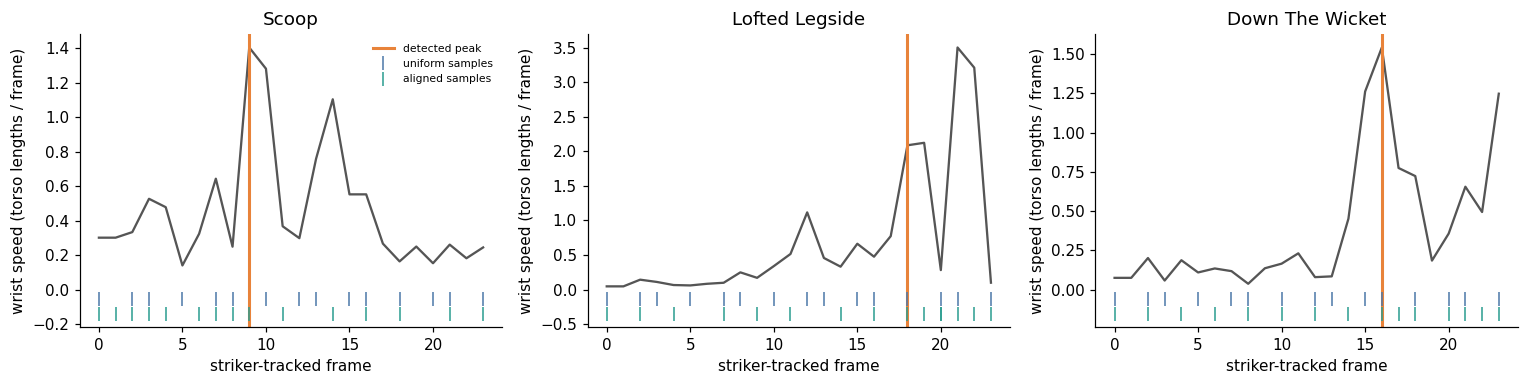
\includegraphics[width=0.98\columnwidth]{fig_phase_alignment.png}
\caption{\textbf{Wrist-Velocity Impact Phase Alignment in Approach 3.} Detecting the peak wrist speed $t_{\text{imp}}$ aligns every video into 7 setup frames, 12 impact frames, and 6 follow-through frames.}
\label{fig:phase_align}
\end{figure}

\paragraph{2. 68-D Biomechanical Pose Descriptor and Wrist-Velocity Impact Alignment (Why: Synchronizing Shot Timing).}
Raw pixel coordinates depend on camera zoom. We first linearly interpolate any low-confidence joints ($c_{t,j} < 0.25$) across valid frames, and then normalize all 17 COCO body joints by centering them at the hip midpoint $\mathbf{p}_{\text{hip}}$ and dividing by the clip-median torso length $L_{\text{torso}} = \text{median}_t \|\mathbf{p}_{\text{sho}}(t) - \mathbf{p}_{\text{hip}}(t)\|_2$. Concatenating the 34-D hip-centered coordinates, 17-D joint confidences, 8-D interior limb angles (elbows, shoulders, hips, knees), 1-D torso lean angle, 4-D normalized wrist velocities, 2-D hip velocity, and 2-D cumulative hip displacement from the first frame (which directly captures the batter advancing down the pitch in \textit{Down The Wicket}) yields a compact \textbf{68-D biomechanical pose vector} per frame.

To fix temporal misalignment across clips, we smooth the striker's maximum wrist speed $v_{\text{wrist}}(t)$ and locate the impact proxy frame $t^* = \arg\max_{t \in [0.2N, 0.85N]} v_{\text{wrist}}(t)$ (\Cref{fig:phase_align}). We then sample $K=15$ frames using a piecewise-linear time warp so that the impact frame $t^*$ always lands exactly on slot $k_{\text{peak}} = 8$, giving 8 pre-impact setup/downswing frames and 6 post-impact follow-through frames.

\paragraph{3. Handedness-Invariant EfficientNetV2-S + Modality-Dropout Dual-GRU Fusion.}
For visual features, we pass both the original and horizontally mirrored $224\times224$ segmentation-overlaid striker crops through a frozen \texttt{EfficientNetV2-S} backbone with $2\times2$ adaptive average pooling, yielding a $1280\times2\times2 = 5120$-D visual vector per frame. Both the visual stream ($15\times5120$, LayerNorm + 128-unit GRU) and the z-score normalized pose stream ($15\times68 \rightarrow \text{Linear}(128) \rightarrow$ 128-unit GRU) are flattened across the $K=15$ steps and concatenated into a 3840-D representation passed through BatchNorm and a 1024-unit classification head. During training, we apply horizontal mirror augmentation (swapping left/right COCO joints in the pose stream) and \textbf{stochastic modality dropout} ($p=0.15$) so the fusion network relies on both appearance and biomechanics.
